\documentclass[tikz,border=9pt]{standalone}
\usepackage[T1]{fontenc}
\usepackage{lmodern}
\usepackage{amsmath,amssymb}
\usetikzlibrary{arrows.meta,positioning}
\definecolor{ink}{HTML}{203044}
\definecolor{line}{HTML}{798899}
\definecolor{front}{HTML}{EAF1F8}
\definecolor{side}{HTML}{B9CDE1}
\definecolor{top}{HTML}{DCE7F1}
\definecolor{panel}{HTML}{F4F6F8}
\definecolor{red}{HTML}{F2DAD8}
\definecolor{green}{HTML}{DCEBD9}
\definecolor{blue}{HTML}{DCE5F3}
\begin{document}
\pagecolor{white}
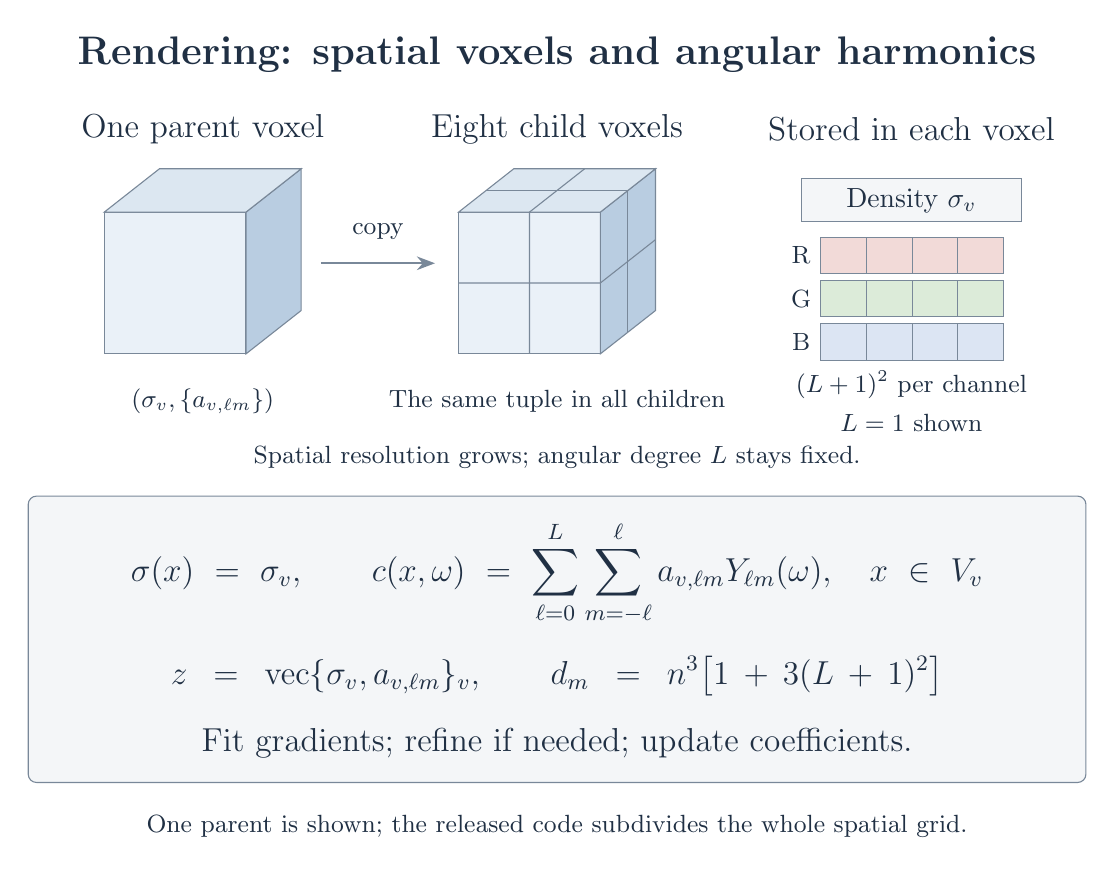
\begin{tikzpicture}[
  text=ink,
  arrow/.style={-{Stealth[length=2.3mm]},draw=line,line width=.8pt},
  label/.style={font=\large,align=center},
  box/.style={draw=line,rounded corners=3pt,fill=panel,
    text width=12.8cm,align=center,inner sep=9pt,font=\large}
]
  \node[font=\Large\bfseries] at (4.5,3.8)
    {Rendering: spatial voxels and angular harmonics};
  \node[label] at (0,2.85) {One parent voxel};
  \node[label] at (4.5,2.85) {Eight child voxels};
  \node[label] at (9,2.85) {Stored in each voxel};

  \foreach \shift in {0,4.5}{
    \filldraw[fill=front,draw=line] ({\shift-1.25},0)
      rectangle ({\shift+.55},1.8);
    \filldraw[fill=side,draw=line] ({\shift+.55},0)
      -- ({\shift+1.25},.55) -- ({\shift+1.25},2.35)
      -- ({\shift+.55},1.8) -- cycle;
    \filldraw[fill=top,draw=line] ({\shift-1.25},1.8)
      -- ({\shift-.55},2.35) -- ({\shift+1.25},2.35)
      -- ({\shift+.55},1.8) -- cycle;
  }
  \draw[draw=line] (4.15,0) -- (4.15,1.8) -- (4.85,2.35);
  \draw[draw=line] (3.25,.9) -- (5.05,.9) -- (5.75,1.45);
  \draw[draw=line] (5.4,.275) -- (5.4,2.075) -- (3.6,2.075);
  \draw[arrow] (1.5,1.15) -- (2.95,1.15)
    node[midway,above=5pt,font=\small] {copy};
  \node[label,font=\small] at (0,-.6) {\((\sigma_v,\{a_{v,\ell m}\})\)};
  \node[label,font=\small] at (4.5,-.6) {The same tuple in all children};

  \node[draw=line,fill=panel,minimum width=2.8cm,minimum height=.5cm]
    at (9,1.95) {Density \(\sigma_v\)};
  \foreach \y/\col/\channel in {1.25/red/R,.7/green/G,.15/blue/B}{
    \node[font=\small] at (7.6,\y) {\channel};
    \foreach \i in {0,1,2,3}{
      \filldraw[fill=\col,draw=line]
        ({7.85+.58*\i},{\y-.23})
        rectangle ({8.43+.58*\i},{\y+.23});
    }
  }
  \node[label,font=\small] at (9,-.6)
    {\((L+1)^2\) per channel\\[3pt]\(L=1\) shown};
  \node[font=\small] at (4.5,-1.32)
    {Spatial resolution grows; angular degree \(L\) stays fixed.};

  \node[box,anchor=north] (summary) at (4.5,-1.8) {
    \(\displaystyle
      \sigma(x)=\sigma_v,\qquad
      c(x,\omega)=\sum_{\ell=0}^{L}\sum_{m=-\ell}^{\ell}
        a_{v,\ell m}Y_{\ell m}(\omega),\quad x\in V_v
    \)\\[10pt]
    \(\displaystyle
      z=\operatorname{vec}\{\sigma_v,a_{v,\ell m}\}_v,
      \qquad d_m=n^3\bigl[1+3(L+1)^2\bigr]
    \)\\[10pt]
    Fit gradients; refine if needed; update coefficients.
  };
  \node[label,font=\small,below=8pt of summary]
    {One parent is shown; the released code subdivides the whole spatial grid.};
\end{tikzpicture}
\end{document}
